% Provenance (never printed): old seconde/premiere S material on water as a
% resource (stocks and flows of the water cycle, residence times, groundwater,
% overuse as a physical fact); see sources/book2/PROVENANCE.md. Residence
% times are computed in figdata/grade-10/residence_times.py, the Aral Sea
% budget in figdata/grade-10/aral_sea.py.
\chapter{Os recursos de água doce}\label{ch:g10:freshwater-resources}

Em 1960, o Mar de Aral, nos desertos da Ásia Central, era o quarto maior
lago do mundo. Dois grandes rios, alimentados pela neve e pela chuva de
montanhas distantes, corriam para ele; nenhum saía dele. Nos anos 1960, a
água desses rios foi desviada para irrigar o deserto. Os satélites
acompanharam o que veio depois: o lago se partiu em pedaços, e a maior parte
do seu leito é hoje terra seca. A causa, de longe a principal, não foi uma
mudança do clima, mas a irrigação: o lago recebia muito menos água do que a
evaporação lhe tirava a cada ano. Este capítulo conta a água da Terra, onde
ela está armazenada e com que rapidez se move, e mostra que um recurso de
água é antes de tudo um \omterm{def:g10:freshwater-resources:stock}{fluxo}: quando se tira de um reservatório mais do que
entra nele, o reservatório se esvazia, num ritmo que um balanço simples
prevê.
% ledger: nasa:aral, gaybullaev:aral-1960, micklin:aral

\begin{omfigure}
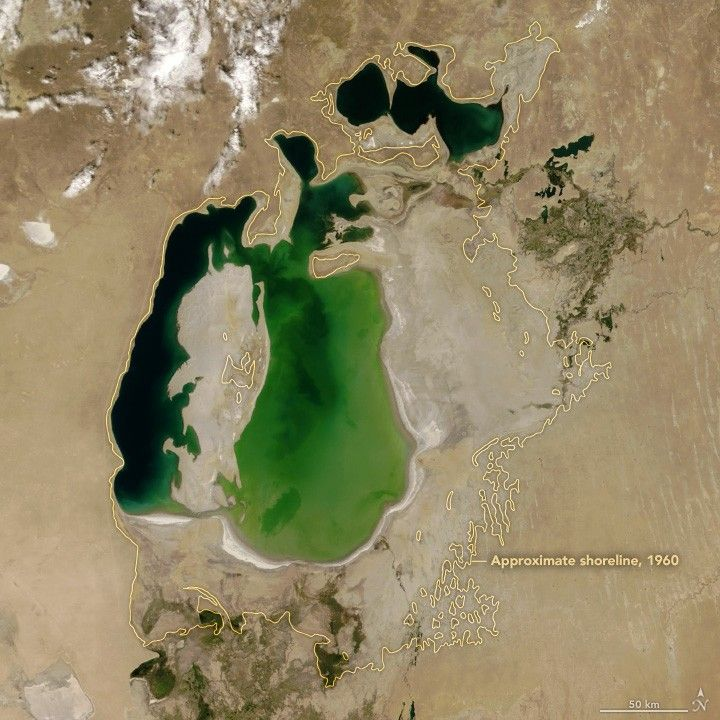
\includegraphics[width=0.47\linewidth]{images/book2/g10-nasa-aral-2000.jpg}\hspace{0.03\linewidth}%
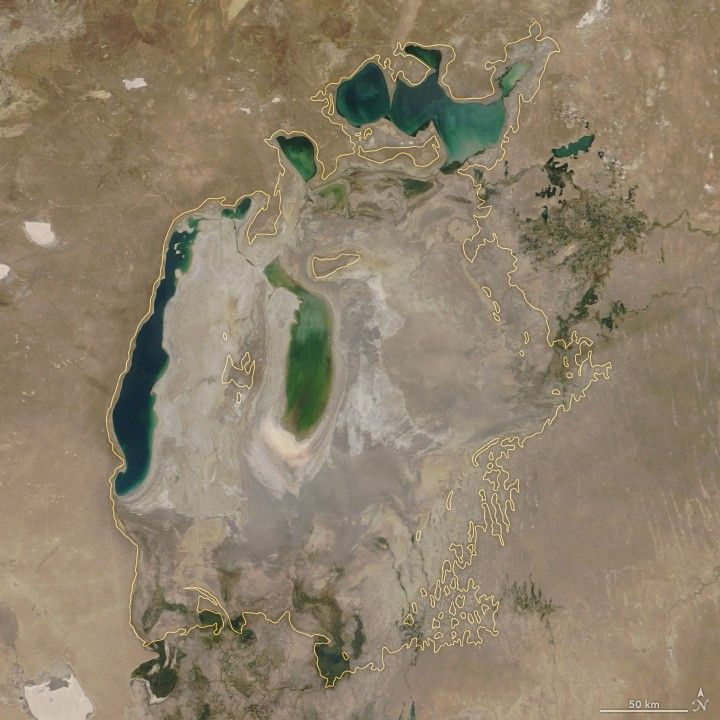
\includegraphics[width=0.47\linewidth]{images/book2/g10-nasa-aral-2018.jpg}

{\small O Mar de Aral visto pelo instrumento MODIS do satélite Terra da
NASA em agosto de 2000 (à esquerda) e em agosto de 2018 (à direita); a linha
amarela é a linha de costa aproximada de 1960. A barra de escala mede
\qty{50}{km}. Imagens: NASA Earth Observatory.}
\end{omfigure}

\begin{recall}
O ciclo da água move a água entre o oceano, o ar e as terras emersas:
evaporação, condensação em nuvens, precipitação, escoamento; a massa total
de água se conserva (os livros de física). As rochas com poros ligados entre
si são permeáveis; abaixo do lençol freático, os seus poros estão cheios de
água, e uma camada que retém e deixa passar água suficiente para alimentar
poços é um aquífero (Livro 1, 6º ano). A maior parte da água da Terra é
água salgada (Livro 1, 2º ano). Um rio leva embora a água da sua \omterm{def:g10:drainage-basins:drainage-basin}{bacia
hidrográfica}; a sua \omterm{def:g10:drainage-basins:discharge}{vazão} é um volume por segundo
(\cref{ch:g10:drainage-basins}).
\end{recall}

\section{Onde está a água}

A Terra contém cerca de 1.39 bilhão de quilômetros cúbicos de água. Quase
toda ela está no oceano; apenas \qty{2.5}{\percent} é doce. E a maior parte
dessa água doce está fora de alcance: mais de dois terços dela estão
congelados nas calotas de gelo e nas geleiras, e quase um terço fica no
subsolo.
% ledger: usgs:water-stocks

\begin{center}
\small
\begin{tabular}{|l|r|r|}
\hline
\textbf{reservatório} & \textbf{volume (\unit{km^3})} & \textbf{parte da água doce} \\ \hline
oceanos, mares e baías & \num{1338000000} & (salgada) \\ \hline
calotas de gelo, geleiras e neve permanente & \num{24064000} & \qty{68.7}{\percent} \\ \hline
água subterrânea doce & \num{10530000} & \qty{30.1}{\percent} \\ \hline
gelo do solo e permafrost & \num{300000} & \qty{0.86}{\percent} \\ \hline
lagos de água doce & \num{91000} & \qty{0.26}{\percent} \\ \hline
umidade do solo & \num{16500} & \qty{0.05}{\percent} \\ \hline
atmosfera & \num{12900} & \qty{0.04}{\percent} \\ \hline
rios & \num{2120} & \qty{0.006}{\percent} \\ \hline
\end{tabular}

{\small Uma estimativa da água do mundo, segundo Shiklomanov (1993), pelo
U.S. Geological Survey. A água subterrânea salgada (\num{12870000}~\unit{km^3})
e os lagos salgados ficaram de fora.}
\end{center}
% ledger: usgs:water-stocks

Os rios e os lagos de água doce, de onde as pessoas tiram a maior parte da
água que usam, contêm juntos menos de um centésimo de um por cento de toda a
água. No entanto, os rios nunca secam por muito tempo: eles não são um
\omterm{def:g10:freshwater-resources:stock}{estoque}, mas um \omterm{def:g10:freshwater-resources:stock}{fluxo}, reabastecido a cada chuva.

\section{Estoques e fluxos}

\begin{definition}[Estoque; fluxo]\label{def:g10:freshwater-resources:stock}
Num balanço de água, um \emph{estoque}\index{estoque (de agua)@estoque (de água)} é a quantidade de
água contida num reservatório --- o oceano, o ar, o gelo, um aquífero, um
lago --- num dado momento, como um volume ou uma massa. Um
\emph{fluxo}\index{fluxo (de agua)@fluxo (de água)} é a quantidade que passa de um reservatório para
outro por unidade de tempo, por exemplo em quilômetros cúbicos por ano.
\end{definition}

Um \omterm{def:g10:freshwater-resources:stock}{estoque} só muda por meio dos seus \omterm{def:g10:freshwater-resources:stock}{fluxos}: o que entra menos o que sai.
Quando os dois são iguais, o \omterm{def:g10:freshwater-resources:stock}{estoque} está em \emph{regime estacionário}: ele
permanece o mesmo, embora a sua água esteja sempre sendo substituída.

\begin{omfigure}
\begin{tikzpicture}[font=\footnotesize, >={Stealth[length=6pt]}]
  % ocean, land, atmosphere
  \fill[omSea] (0,0) rectangle (6.4,1.6);
  \fill[omLithAlluv] (6.4,0) -- (6.4,1.6) -- (8.2,2.1) -- (10.4,2.6) -- (12,2.9) -- (12,0) -- cycle;
  \fill[omLithSand!60] (6.4,0) -- (12,0) -- (12,1.0) -- (6.4,0.7) -- cycle;
  \draw[black!50] (6.4,1.6) -- (8.2,2.1) -- (10.4,2.6) -- (12,2.9);
  \fill[omIce] (10.6,2.65) -- (11.3,3.35) -- (12,2.9) -- cycle;
  \node[align=center] at (3.2,0.75) {\textbf{oceano}\\\num{1335040}};
  \node[align=center] at (9.3,1.35) {umidade do solo 122\\lagos e rios 178};
  \node[align=center] at (9.3,0.35) {água subterrânea \num{15300}};
  \node[align=center] at (11.2,2.25) {gelo\\\num{26350}};
  % atmosphere
  \draw[black!30, rounded corners=8pt, fill=omWxCloud] (1.0,4.6) rectangle (11.0,5.6);
  \node[align=center] at (6.0,5.1) {\textbf{atmosfera} 12.7};
  % fluxes
  \draw[->, omProp, line width=1.4pt] (1.4,1.7) -- node[left, align=right] {evaporação\\413} (1.4,4.5);
  \draw[->, omWxRain, line width=1.4pt] (4.4,4.5) -- node[pos=0.3, right, align=left] {precipitação\\373} (4.4,1.7);
  \draw[->, omWxRain, line width=1.4pt] (7.6,4.5) -- node[pos=0.7, left, align=right] {precipitação\\113} (7.6,2.05);
  \draw[->, omProp, line width=1.4pt] (10.0,2.6) -- node[right, align=left] {evaporação e\\transpiração 73} (10.0,4.5);
  \draw[->, black!60, line width=1.2pt] (4.9,5.85) -- node[above] {vapor de água levado sobre as terras: 40} (7.4,5.85);
  \draw[->, omRiver, line width=1.4pt] (7.6,1.2) -- node[above, inner sep=2pt] {escoamento 40} (6.0,1.2);
\end{tikzpicture}

{\small O ciclo global da água dos anos 1990 (esquema; fora de escala).
\omterm{def:g10:freshwater-resources:stock}{Estoques} em milhares de \unit{km^3}, \omterm{def:g10:freshwater-resources:stock}{fluxos} em milhares de \unit{km^3} por
ano. Segundo Trenberth e colaboradores (2007). As estimativas dos \omterm{def:g10:freshwater-resources:stock}{estoques}
diferem de um estudo para outro: compare a água subterrânea e o gelo daqui
com a tabela acima.}
\end{omfigure}
% ledger: trenberth:water-cycle

O ciclo está equilibrado. A cada ano, o oceano perde \num{413000}~\unit{km^3}
por evaporação e recebe de volta \num{373000} como chuva e neve e
\num{40000} dos rios. O ar recebe $413\,000 + 73\,000 = \num{486000}$~\unit{km^3}
e devolve $373\,000 + 113\,000$, a mesma quantidade. As terras emersas
recebem \num{113000}~\unit{km^3} de precipitação; \num{73000} voltam ao ar
por evaporação e pelas folhas das plantas, e os \num{40000} restantes
escoam para o mar, pelos rios e pelo subsolo.
% ledger: trenberth:water-cycle

\begin{definition}[Água doce renovável]\label{def:g10:freshwater-resources:renewable}
A \emph{água doce renovável}\index{agua doce renovavel@água doce renovável}
de uma região é o \omterm{def:g10:freshwater-resources:stock}{fluxo} de água doce renovado a cada ano pela precipitação,
que a atravessa como escoamento nos rios e como água subterrânea. É um
\omterm{def:g10:freshwater-resources:stock}{fluxo}, em quilômetros cúbicos por ano, e não um \omterm{def:g10:freshwater-resources:stock}{estoque}.
\end{definition}

Para todas as terras emersas da Terra, são os \num{40000}~\unit{km^3} que
chegam ao mar a cada ano. Uma região pode usar a sua água renovável ano após
ano sem que ela falte. O que ela tira além disso só pode vir de um \omterm{def:g10:freshwater-resources:stock}{estoque},
que então diminui.

\section{O tempo de residência}

Quanto tempo uma molécula de água fica num reservatório? Algumas saem logo,
outras ficam muito mais; mas, em média, a resposta decorre apenas do \omterm{def:g10:freshwater-resources:stock}{estoque}
e do \omterm{def:g10:freshwater-resources:stock}{fluxo}.

\begin{definition}[Tempo de residência]\label{def:g10:freshwater-resources:residence-time}
O \emph{tempo de residência}\index{tempo de residencia@tempo de residência}
da água num reservatório é o tempo médio que a água passa nele entre a
entrada e a saída.
\end{definition}

\begin{proposition}[Tempo de residência, estoque e fluxo]\label{prop:g10:freshwater-resources:residence}
Para um reservatório em regime estacionário, que contém um \omterm{def:g10:freshwater-resources:stock}{estoque} $S$
atravessado por um \omterm{def:g10:freshwater-resources:stock}{fluxo} $F$ (de entrada e de saída), o \omterm{def:g10:freshwater-resources:residence-time}{tempo de residência}
é
\[
T = \frac{S}{F}.
\]
\end{proposition}

\begin{proof}
Em regime estacionário, um volume $F$ entra e um volume $F$ sai a cada ano,
enquanto o \omterm{def:g10:freshwater-resources:stock}{estoque} permanece $S$. Depois de um tempo $S/F$, entrou um volume
$F \times S/F = S$: tanto quanto o reservatório inteiro contém. Em média, a
água presente no início foi então substituída, de modo que a água fica $S/F$
no reservatório.
\end{proof}

\begin{example}[A água no ar]\label{ex:g10:freshwater-resources:atmosphere}
A atmosfera contém \num{12700}~\unit{km^3} de água, e
\num{486000}~\unit{km^3} caem dela a cada ano como chuva e neve. O seu
\omterm{def:g10:freshwater-resources:residence-time}{tempo de residência} é $12\,700/486\,000 \approx \num{0.026}$ ano, cerca de
\num{9.5} dias: a água do ar é renovada a cada uma ou duas semanas. Uma nuvem
que chove hoje é feita de água que deixou o oceano ou o solo há alguns
dias.
\end{example}
% ledger: trenberth:water-cycle (t_atmosphere_days 9.5 in figdata/grade-10/residence_times.py)

O mesmo cálculo dá cerca de \num{19} dias para a água nos leitos dos rios
($2120$~\unit{km^3} levados por \num{40000}~\unit{km^3} por ano), alguns
anos para os lagos e os rios juntos, e cerca de \num{3200} anos para o
oceano ($1\,335\,040/413$ mil~\unit{km^3}). A água subterrânea pode ser
ainda mais lenta: a água mais profunda de alguns aquíferos tem centenas de
milhares de anos.
% ledger: trenberth:water-cycle, usgs:water-stocks, sturchio:nubian-age

\begin{omfigure}
\begin{tikzpicture}
\begin{axis}[omrecord, xbar, xmode=log, log origin=infty, width=0.74\linewidth, height=5.6cm,
  xmin=1, xmax=1e9, ymin=-0.6, ymax=4.6, bar width=11pt,
  ytick={0,1,2,3,4}, yticklabels={atmosfera, rios, {lagos e rios}, oceano, {água subterrânea profunda (idade)}},
  xtick={1,30.44,365.25,36525,3652500,365250000}, xticklabels={1 dia, 1 mês, 1 ano, 100 anos, \num{10000} anos, 1 milhão de anos},
  xticklabel style={font=\scriptsize, rotate=25, anchor=north east}, yticklabel style={font=\small},
  xlabel={tempo de residência (escala logarítmica)}, label style={font=\small}, xmajorgrids]
\addplot[fill=omDef!45, draw=omDef!80!black] table[x=days, y=idx] {figdata/out/grade-10-residence_times-times.dat};
\draw[fill=omProp!45, draw=omProp!80!black] (axis cs:73050000,3.75) rectangle (axis cs:365250000,4.25);
\node[anchor=west, font=\scriptsize] at (axis cs:9.5,0) {\num{9.5} dias};
\node[anchor=west, font=\scriptsize] at (axis cs:19.4,1) {\num{19} dias};
\node[anchor=west, font=\scriptsize] at (axis cs:1625,2) {\num{4.5} anos};
\node[anchor=west, font=\scriptsize] at (axis cs:1180690,3) {\num{3200} anos};
\node[anchor=east, font=\scriptsize] at (axis cs:73050000,4) {\num{200000} a 1 milhão de anos};
\end{axis}
\end{tikzpicture}

{\small \omterm{def:g10:freshwater-resources:residence-time}{Tempos de residência} da água, calculados como \omterm{def:g10:freshwater-resources:stock}{estoque} dividido por
\omterm{def:g10:freshwater-resources:stock}{fluxo} a partir do ciclo global da água (azul), e a idade medida da água
subterrânea profunda sob o Saara oriental (laranja). Eixo logarítmico: a
partir de um ano, cada degrau marcado vale cem vezes o anterior. Dados:
Trenberth e colaboradores (2007); U.S. Geological Survey; Sturchio e
colaboradores (2004).}
\end{omfigure}
% values computed in figdata/grade-10/residence_times.py

O \omterm{def:g10:freshwater-resources:residence-time}{tempo de residência} mede a rapidez com que um reservatório se recupera. A
água tirada de um rio é reposta em dias; um lago poluído ou esvaziado leva
anos; uma água subterrânea que levou milhares de anos para se acumular não
se renova, na escala de uma vida humana.

\begin{method}[Um balanço de água]\label{met:g10:freshwater-resources:budget}
\begin{enumerate}
  \item Escolha o reservatório: um lago, um aquífero, uma bacia, o ar.
  \item Liste cada \omterm{def:g10:freshwater-resources:stock}{fluxo} que entra nele (rios, chuva, infiltração) e que sai
        dele (rios, evaporação, bombeamento), na mesma unidade.
  \item A variação do \omterm{def:g10:freshwater-resources:stock}{estoque} por ano é a soma das entradas menos a soma das
        saídas.
  \item Se o \omterm{def:g10:freshwater-resources:stock}{estoque} não muda, as entradas igualam as saídas, e o \omterm{def:g10:freshwater-resources:residence-time}{tempo de
        residência} é o \omterm{def:g10:freshwater-resources:stock}{estoque} dividido por uma ou outra.
\end{enumerate}
\end{method}

\section{Os aquíferos como reservatórios}

A chuva que se infiltra no solo e chega ao lençol freático \emph{recarrega}
o aquífero abaixo. A água então se desloca devagar pelos poros da rocha, em
direção às fontes, aos rios ou ao mar. Onde uma camada permeável mergulha
sob uma camada impermeável, como a argila, a sua água fica
\emph{confinada}: ela só é alimentada onde a camada aflora, o que pode ser
muito longe.

\begin{omfigure}
\begin{tikzpicture}[font=\footnotesize, >={Stealth[length=5pt]}]
  % layers dipping to the right
  \fill[lith shale] (0,0) -- (12,0) -- (12,0.8) -- (0,2.4) -- cycle;
  \fill[lith sandstone] (0,2.4) -- (12,0.8) -- (12,2.2) -- (2.2,3.5) -- (0,3.8) -- cycle;
  \fill[lith shale] (2.2,3.5) -- (12,2.2) -- (12,3.4) -- (3.6,3.9) -- cycle;
  % ground surface
  \draw[line width=0.8pt, brown!60!black] (0,3.8) -- (1.2,4.0) -- (2.2,3.9) -- (3.6,3.9) -- (6,3.6) -- (9,3.5) -- (12,3.4);
  \fill[omLithAlluv] (0,3.8) -- (1.2,4.0) -- (2.2,3.9) -- (2.2,3.5) -- (0,3.8) -- cycle;
  \fill[omLithAlluv] (2.2,3.9) -- (3.6,3.9) -- (2.2,3.5) -- cycle;
  \fill[omLithAlluv] (3.6,3.9) -- (6,3.6) -- (9,3.5) -- (12,3.4) -- (3.6,3.9) -- cycle;
  % water table in the unconfined part
  \draw[omDef, line width=1pt, dashed] (0,3.3) .. controls (1.0,3.35) and (1.8,3.2) .. (2.6,3.45);
  \node[anchor=south west, text=omDef, fill=white, fill opacity=0.8, text opacity=1, inner sep=1pt] at (0.05,2.75) {lençol freático};
  % rain and recharge
  \foreach \x in {0.35,0.65,0.95,1.25} \draw[omWxRain, thick] (\x,4.9) -- (\x-0.15,4.4);
  \node[anchor=south, text=omWxRain] at (0.7,4.95) {chuva: recarga};
  % flow arrows in the aquifer
  \draw[->, omDef, line width=1.1pt] (2.0,2.85) -- (4.4,2.55);
  \draw[->, omDef, line width=1.1pt] (5.4,2.4) -- (7.8,2.1);
  \draw[->, omDef, line width=1.1pt] (8.8,1.95) -- (11.2,1.65);
  % wells
  \draw[black!70, line width=1.6pt] (1.95,3.95) -- (1.95,2.9);
  \node[anchor=south] at (1.95,4.0) {poço};
  \draw[black!70, line width=1.6pt] (7.0,3.55) -- (7.0,1.9);
  \node[anchor=south] at (7.0,3.6) {poço};
  % labels
  \node[align=center, fill=white, fill opacity=0.85, text opacity=1, inner sep=1.5pt] at (1.5,0.8) {argila impermeável};
  \node[align=center, fill=white, fill opacity=0.85, text opacity=1, inner sep=1.5pt] at (8.6,2.95) {argila impermeável};
  \node[anchor=north, align=center] at (1.6,-0.1) {aquífero livre:\\área de recarga};
  \node[anchor=north, align=center] at (6.4,-0.1) {aquífero confinado};
  \node[anchor=north, align=center] at (10.6,-0.1) {água antiga, longe da\\área de recarga};
\end{tikzpicture}

{\small Um aquífero num arenito permeável (esquema). A chuva o recarrega
onde ele aflora; ali, o lençol freático está livre para subir e descer. Mais
adiante, sob a argila, o aquífero é confinado, e a sua água desce devagar ao
longo da camada: quanto mais longe da área de recarga, mais antiga a água.}
\end{omfigure}

\begin{definition}[Água subterrânea fóssil]\label{def:g10:freshwater-resources:fossil-groundwater}
A \emph{água subterrânea fóssil}\index{agua subterranea fossil@água subterrânea fóssil} é a água subterrânea
que entrou no seu aquífero há muito tempo, muitas vezes sob um clima mais
úmido, e que a recarga atual não renova na escala das vidas humanas.
\end{definition}

Sob o Saara oriental fica um vasto aquífero de arenito. A sua água mais
profunda, datada pelo decaimento de uma forma radioativa rara do criptônio,
tem de \num{200000} a um milhão de anos. Ela entrou devagar a partir de uma
área de recarga no sudoeste do Egito, e a sua química mostra que caiu como
chuva durante períodos úmidos passados das eras glaciais, quando o ar úmido
do Atlântico chegava à região. Bombeada hoje, essa água é um \omterm{def:g10:freshwater-resources:stock}{estoque} que se
esgota, e não um \omterm{def:g10:freshwater-resources:stock}{fluxo}.
% ledger: sturchio:nubian-age

Quando o bombeamento supera a recarga, o lençol freático desce. Nas High
Plains, no centro dos Estados Unidos, o aquífero sob umas \num{175000}
milhas quadradas (\qty{453000}{km^2}) é bombeado para a irrigação desde
cerca de 1950. Em 2015, o seu nível de água tinha descido \qty{4.8}{m} em
média, e até \qty{71}{m} (234 pés) em alguns poços; o aquífero tinha perdido
cerca de \num{273} milhões de acres-pés de água, uns \qty{340}{km^3}.
% ledger: mcguire:high-plains (1 acre-foot = 1233.5 m3)

\begin{omfigure}
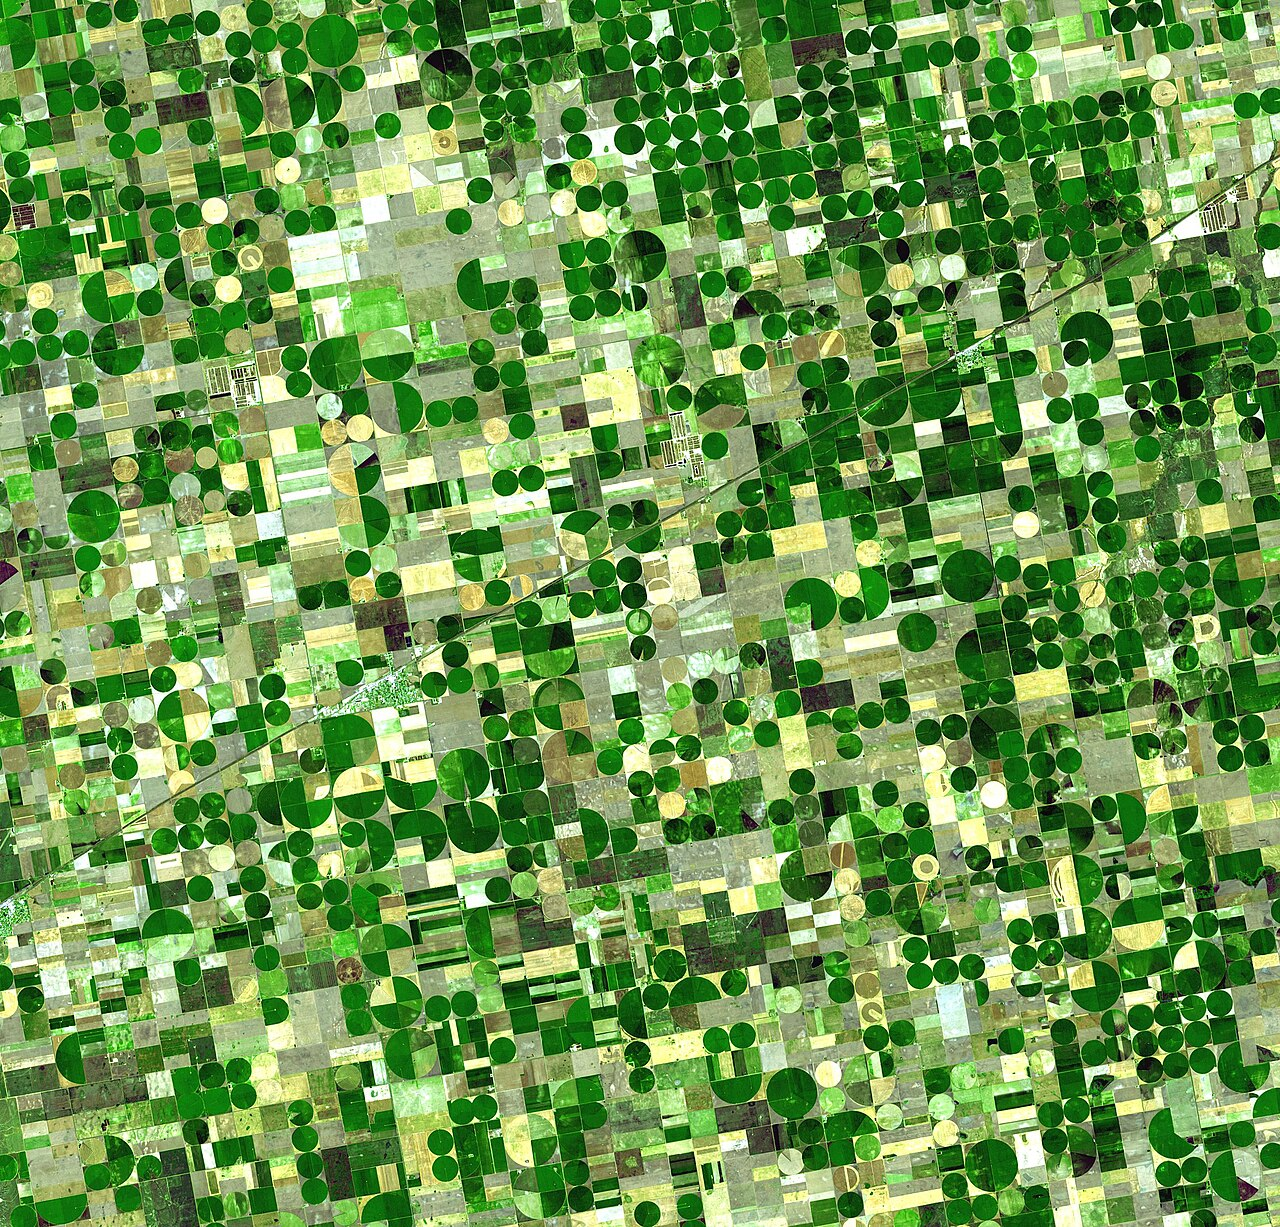
\includegraphics[width=0.5\linewidth]{images/book2/g10-nasa-kansas-center-pivot.jpg}

{\small Campos irrigados perto de Sublette, no Kansas, vistos pelo
instrumento ASTER do satélite Terra da NASA em junho de 2001 (cerca de
\qty{37}{km} de lado a lado). Cada círculo é um campo regado por um longo
braço aspersor que gira em torno do seu centro; os círculos têm \num{800} e
\qty{1600}{m} de diâmetro. Imagem: NASA (domínio público).}
\end{omfigure}

A água subterrânea não pode ser vista do espaço, mas pode ser pesada: dois
satélites que voam um atrás do outro sentem as pequenas variações da atração
da Terra causadas pela massa de água que vai e vem abaixo deles, e mapeiam
onde o \omterm{def:g10:freshwater-resources:stock}{estoque} de água nas terras emersas sobe e desce de mês em mês.

\begin{omfigure}
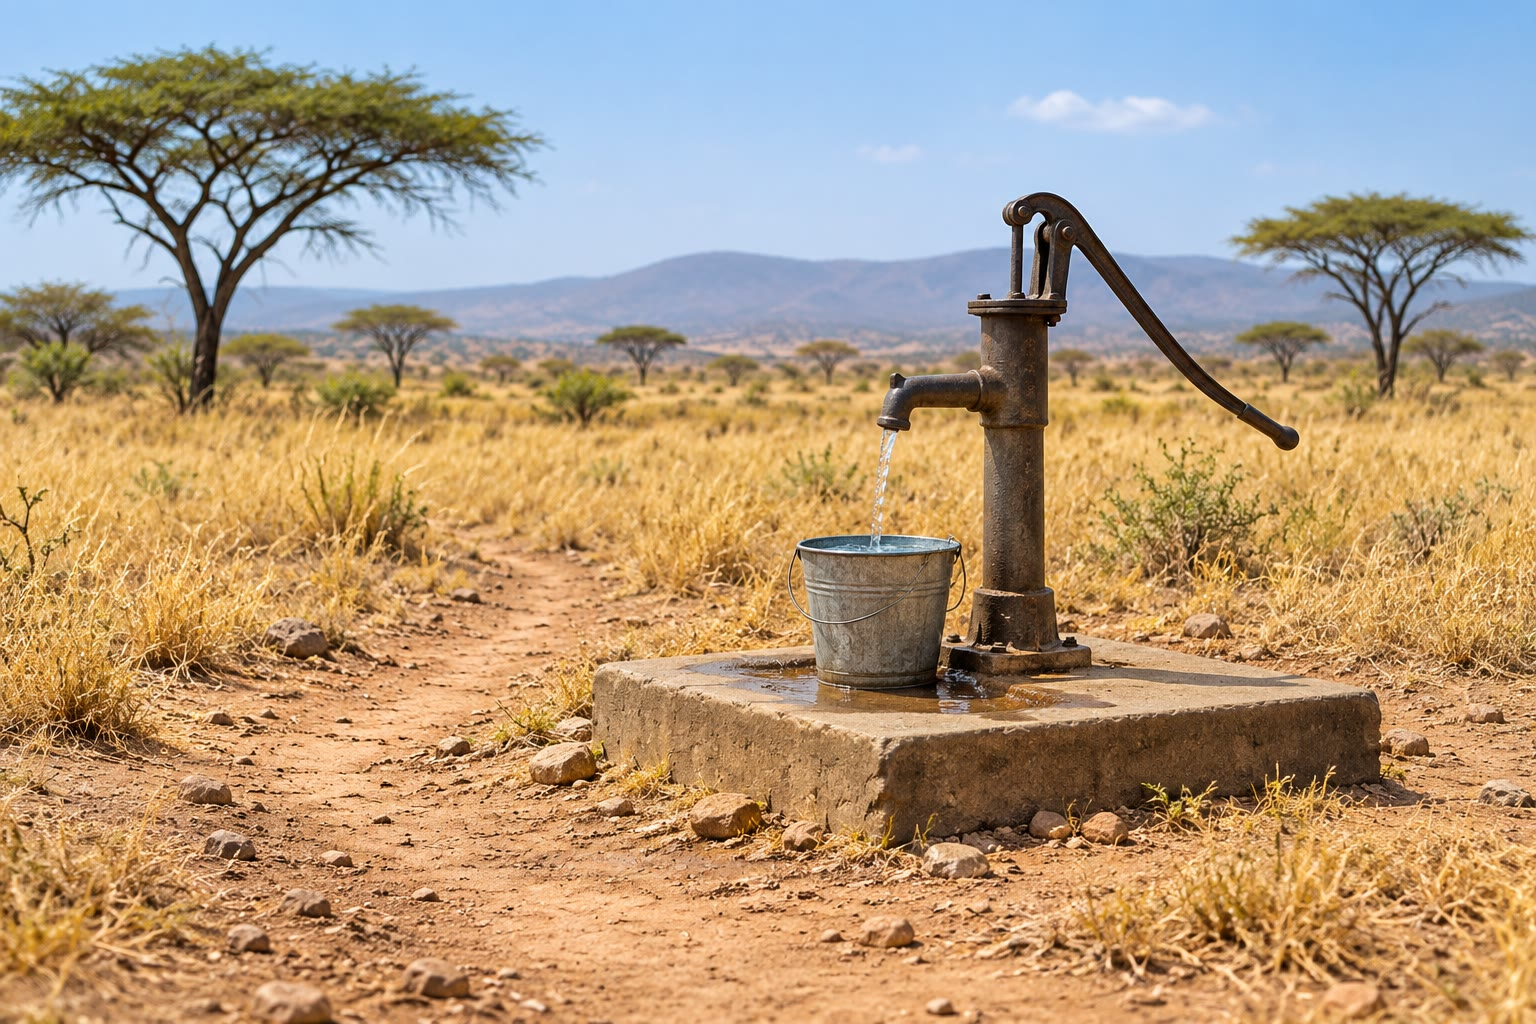
\includegraphics[width=0.55\linewidth]{images/book2/ai/g10-hand-pump-well.jpg}

{\small Uma bomba manual num poço numa paisagem seca: a água tirada aqui vem
do subsolo, fora do alcance da estação seca.}
\end{omfigure}

\section{O uso excessivo como fato físico}

O Mar de Aral não tem saída: a água dos seus dois rios, o Amu Dária e o Sir
Dária, só sai por evaporação. Em 1960, ele cobria \qty{68000}{km^2},
continha \qty{1093}{km^3} e a sua água tinha \qty{10}{g} de sal por litro.
Nesse ano, a evaporação retirou \qty{71.1}{km^3}, e a chuva sobre o lago
trouxe \qty{9.4}{km^3}: para manter o seu nível, o lago precisava de
$71.1 - 9.4 = \qty{61.7}{km^3}$ por ano vindos dos seus rios.
% ledger: gaybullaev:aral-1960, gaybullaev:aral-table

A partir dos anos 1960, os rios foram desviados para irrigar o deserto, e
quase nada da sua água chegava ao lago: nos anos 1970 e 1980, muitas vezes
menos de \qty{2}{km^3} por ano. A evaporação continuou, e o lago começou a
encolher. O seu balanço dita a que velocidade. A evaporação tira uma camada
de água cuja espessura depende do clima, aqui cerca de um metro por ano
($71.1/68\,000 \approx \qty{0.00105}{km}$). Se a entrada para, o nível desce
mais ou menos isso a cada ano, menos a chuva. À medida que o lago encolhe, a
sua área, e portanto a sua evaporação, também diminuem, e a descida fica
mais lenta; mas ela só para quando a entrada e a evaporação voltam a se
equilibrar.
% ledger: gaybullaev:aral-table (values computed in figdata/grade-10/aral_sea.py)

\begin{omfigure}
\begin{tikzpicture}
\begin{axis}[omrecord, name=vol, width=0.46\linewidth, height=5.4cm, xmin=1955, xmax=2012, ymin=0, ymax=1200,
  xtick={1960,1980,2000}, xticklabel style={/pgf/number format/1000 sep={}}, scaled y ticks=false,
  ylabel={volume (\unit{km^3})}, xlabel={ano}, tick label style={font=\small}, label style={font=\small},
  title={\small volume de água}]
\addplot[omDef, line width=1pt, mark=*, mark size=1.3pt] table[x=year, y=volume] {figdata/out/grade-10-aral_sea-record.dat};
\end{axis}
\begin{axis}[omrecord, at={(vol.east)}, anchor=west, xshift=1.4cm, width=0.46\linewidth, height=5.4cm,
  xmin=1955, xmax=2012, ymin=0, ymax=140, xtick={1960,1980,2000},
  xticklabel style={/pgf/number format/1000 sep={}},
  ylabel={salinidade (\unit{g/L})}, xlabel={ano}, tick label style={font=\small}, label style={font=\small},
  title={\small salinidade}]
\addplot[omProp, line width=1pt, mark=*, mark size=1.3pt] table[x=year, y=salinity] {figdata/out/grade-10-aral_sea-record.dat};
\end{axis}
\end{tikzpicture}

{\small O Mar de Aral de 1960 a 2010: o volume da sua água caiu para um
décimo, enquanto o sal deixado pela evaporação ficou treze vezes mais
concentrado. Dados: Gaybullaev e colaboradores (2012).}
\end{omfigure}
% ledger: gaybullaev:aral-table

Em 2010, o lago continha \qty{98}{km^3}, um décimo do seu volume de 1960,
sobre \qty{14280}{km^2}; a sua salinidade tinha chegado a \qty{130}{g/L},
muito mais salgado que o oceano. O seu nível tinha descido mais de
\qty{20}{m}. Uma poeira salgada é soprada do leito seco. A causa não está
escondida: a entrada do lago foi cortada, mas a sua evaporação não.
% ledger: gaybullaev:aral-table, gaybullaev:aral-1960, micklin:aral, nasa:aral

\section{Exercícios}

\begin{exercise}[$\star$]\label{exo:g10:freshwater-resources:1}
Defina um \omterm{def:g10:freshwater-resources:stock}{estoque}, um \omterm{def:g10:freshwater-resources:stock}{fluxo} e um \omterm{def:g10:freshwater-resources:residence-time}{tempo de residência}, e dê as unidades de
cada um.
\end{exercise}

\begin{exercise}[$\star$]\label{exo:g10:freshwater-resources:2}
Pela tabela da água do mundo: que parte de toda a água é doce? Da água doce,
que partes estão congeladas e no subsolo? Que reservatório contém menos
água?
\end{exercise}

\begin{exercise}[$\star$]\label{exo:g10:freshwater-resources:3}
Defina a \omterm{def:g10:freshwater-resources:renewable}{água doce renovável} e a \omterm{def:g10:freshwater-resources:fossil-groundwater}{água subterrânea fóssil}. Por que a
primeira é um \omterm{def:g10:freshwater-resources:stock}{fluxo} e a segunda, um \omterm{def:g10:freshwater-resources:stock}{estoque}?
\end{exercise}

\begin{exercise}[$\star$]\label{exo:g10:freshwater-resources:4}
Quantas vezes mais água contêm os lagos de água doce do mundo
(\num{91000}~\unit{km^3}) do que os seus rios (\num{2120}~\unit{km^3})?
\end{exercise}

\begin{exercise}[$\star$]\label{exo:g10:freshwater-resources:5}
No gráfico dos \omterm{def:g10:freshwater-resources:residence-time}{tempos de residência}, que reservatório renova a sua água mais
depressa, e qual mais devagar? Quantas vezes mais tempo a água fica no
oceano do que no ar?
\end{exercise}

\begin{exercise}[$\star\star$]\label{exo:g10:freshwater-resources:6}
A atmosfera contém \num{12700}~\unit{km^3} de água. Calcule o seu \omterm{def:g10:freshwater-resources:residence-time}{tempo de
residência} a partir da evaporação que entra nela (\num{413000} vindos do
oceano e \num{73000}~\unit{km^3} vindos das terras emersas a cada ano), e
verifique que ele coincide com o \omterm{def:g10:freshwater-resources:residence-time}{tempo de residência} calculado a partir da
precipitação que sai dela.
\end{exercise}

\begin{exercise}[$\star\star$]\label{exo:g10:freshwater-resources:7}
O oceano contém \num{1335040} mil~\unit{km^3} e perde
\num{413} mil~\unit{km^3} por ano por evaporação. Calcule o seu \omterm{def:g10:freshwater-resources:residence-time}{tempo de
residência}. Por que ele é o mesmo se calculado com o que entra nele?
\end{exercise}

\begin{exercise}[$\star\star$]\label{exo:g10:freshwater-resources:8}
Usando os \omterm{def:g10:freshwater-resources:stock}{fluxos} do ciclo global da água, escreva o balanço das terras
emersas: o que cai sobre elas, o que volta ao ar, o que escoa. Que parte da
chuva que cai sobre as terras emersas volta ao ar?
\end{exercise}

\begin{exercise}[$\star\star$]\label{exo:g10:freshwater-resources:9}
O aquífero das High Plains perdeu cerca de \num{273.2} milhões de acres-pés
de água de cerca de 1950 a 2015 (\num{1}~acre-pé = \qty{1233.5}{m^3}).
Converta esse volume em \unit{km^3} e compare-o com o volume do Mar de Aral
em 1987 (\qty{345.6}{km^3}).
\end{exercise}

\begin{exercise}[$\star\star$]\label{exo:g10:freshwater-resources:10}
O nível médio da água do aquífero das High Plains desceu \num{15.8} pés de
cerca de 1950 a 2015 (\num{1}~pé = \qty{0.3048}{m}). Quanto é isso em
metros, e em centímetros por ano?
\end{exercise}

\begin{exercise}[$\star\star$]\label{exo:g10:freshwater-resources:11}
Um aquífero contém \qty{2}{km^3} de água e é recarregado com
\qty{0.01}{km^3} por ano. Qual é o \omterm{def:g10:freshwater-resources:residence-time}{tempo de residência} da sua água? Hoje,
poços bombeiam dele \qty{0.05}{km^3} por ano. Suponha que a recarga
continue e que os poços sejam agora a única saída da água: quanto tempo ele
vai durar?
\end{exercise}

\begin{exercise}[$\star\star\star$]\label{exo:g10:freshwater-resources:12}
Calcule o \omterm{def:g10:freshwater-resources:residence-time}{tempo de residência} da água do Mar de Aral em 1960
(\qty{1093}{km^3}, evaporação de \qty{71.1}{km^3} por ano) e em 2010
(\qty{98.1}{km^3}, evaporação de \qty{11.4}{km^3} por ano). Por que a sua
evaporação diminuiu?
\end{exercise}

\begin{exercise}[$\star\star\star$]\label{exo:g10:freshwater-resources:13}
Um lago sem saída cobre \qty{100}{km^2}. A evaporação retira
\qty{1.2}{m} de água por ano da sua superfície, e a chuva acrescenta
\qty{0.2}{m}.
\begin{enumerate}
  \item Que entrada, em \unit{km^3} por ano, mantém o seu nível estável?
  \item A entrada é reduzida à metade. Quanto o nível desce no primeiro
        ano?
  \item Por que a descida fica mais lenta nos anos seguintes?
\end{enumerate}
\end{exercise}

\begin{exercise}[$\star\star\star$]\label{exo:g10:freshwater-resources:14}
Num deserto, a chuva recarrega um aquífero com \qty{1}{mm} de água por ano.
O aquífero tem \qty{100}{m} de espessura e a água ocupa
\qty{20}{\percent} do seu volume. Quanto tempo a recarga levaria para
enchê-lo? Compare com a idade da água profunda do aquífero do Saara.
\end{exercise}

\begin{exercise}[$\star\star\star$]\label{exo:g10:freshwater-resources:15}
O aquífero das High Plains cobre cerca de \qty{453000}{km^2} e tinha
perdido cerca de \qty{337}{km^3} de água em 2015. Que espessura de água,
espalhada sobre todo o aquífero, isso representa? O seu nível de água desceu
\qty{4.8}{m} em média. Por que a descida do nível da água é maior que a
espessura de água perdida?
\end{exercise}

\section{Problema: o balanço do Mar de Aral}

\begin{problem}[{Problema de fim de semana --- com que rapidez um lago desaparece?}]
\label{pb:g10:freshwater-resources:1}
% ledger: gaybullaev:aral-table, gaybullaev:aral-1960, micklin:aral (values computed in figdata/grade-10/aral_sea.py)
A tabela dá o balanço do Mar de Aral em quatro anos (volumes em
\unit{km^3}, salinidade em gramas de sal por litro). Em 1960, o lago cobria
\qty{68000}{km^2}.
\begin{center}
\small
\begin{tabular}{|c|c|c|c|c|c|}
\hline
ano & entrada dos rios & chuva sobre o lago & evaporação & volume & salinidade \\ \hline
1960 & 42.0 & 9.4 & 71.1 & 1093.0 & 10.0 \\ \hline
1984 & 0.3 & 3.5 & 47.9 & 502.7 & 21.9 \\ \hline
1987 & 1.0 & 6.2 & 36.8 & 345.6 & 25.0 \\ \hline
1989 & 3.1 & 5.3 & 35.3 & 327.2 & 30.0 \\ \hline
\end{tabular}

{\small Dados: Gaybullaev e colaboradores (2012).}
\end{center}

\medskip
\noindent\textbf{Parte I --- O lago em 1960.}
\begin{enumerate}
  \item Qual era a profundidade média do lago em 1960?
  \item Exprima o seu volume em metros cúbicos.
  \item Que massa de sal ele continha, em toneladas?
  \item Qual era o \omterm{def:g10:freshwater-resources:residence-time}{tempo de residência} da sua água, contado com a
        evaporação?
  \item Por que um lago sem saída só pode perder água por evaporação (e por
        infiltração)?
\end{enumerate}

\medskip
\noindent\textbf{Parte II --- Do que o lago precisa.}
\begin{enumerate}[resume]
  \item Que espessura de água a evaporação retirou do lago em 1960, em
        metros?
  \item Que espessura a chuva acrescentou?
  \item Que entrada dos rios teria equilibrado exatamente a evaporação e a
        chuva?
  \item Os dois rios levam em média cerca de \qty{79}{km^3} e
        \qty{37}{km^3} por ano para fora das montanhas. Que parte disso o
        lago precisaria?
\end{enumerate}

\medskip
\noindent\textbf{Parte III --- O lago no fim dos anos 1980.}
\begin{enumerate}[resume]
  \item Escreva o balanço de 1987: entradas, saídas, variação líquida.
  \item Entre 1984 e 1989, o volume caiu de \qty{502.7}{km^3} para
        \qty{327.2}{km^3}. Qual foi a queda média por ano? Compare com o
        balanço de 1987.
  \item Suponha que um quilômetro quadrado de lago perca tanta água por
        evaporação quanto em 1960. Qual era a área do lago em 1987?
  \item Que parte da sua área de 1960 é isso?
  \item Por que a evaporação tinha caído de \qty{71.1}{km^3} para
        \qty{36.8}{km^3}?
  \item Que parte do seu volume de 1960 o lago ainda continha em 1987?
\end{enumerate}

\medskip
\noindent\textbf{Parte IV --- O sal e o nível.}
\begin{enumerate}[resume]
  \item Se todo o sal de 1960 tivesse ficado na água, qual teria sido a
        salinidade em 1987?
  \item A tabela dá \qty{25.0}{g/L}. O que a diferença sugere?
  \item Sem nenhuma entrada e sem chuva alguma, quanto o nível desceria a
        cada ano?
  \item Em 1987, quanto os rios e a chuva acrescentaram, como espessura
        sobre a área da questão 12?
  \item Quanto o nível do Mar de Aral desceu em 1987?
\end{enumerate}
\end{problem}
